\capitulo{4}{Técnicas y herramientas}

%Esta parte de la memoria tiene como objetivo presentar las técnicas metodológicas y las herramientas de desarrollo que se han utilizado para llevar a cabo el proyecto. Si se han estudiado diferentes alternativas de metodologías, herramientas, bibliotecas se puede hacer un resumen de los aspectos más destacados de cada alternativa, incluyendo comparativas entre las distintas opciones y una justificación de las elecciones realizadas. 
%No se pretende que este apartado se convierta en un capítulo de un libro dedicado a cada una de las alternativas, sino comentar los aspectos más destacados de cada opción, con un repaso somero a los fundamentos esenciales y referencias bibliográficas para que el lector pueda ampliar su conocimiento sobre el tema.
Este capitulo muestra las técnicas y herramientas que se han utilizado para la alcanzar los objetivos del proyecto. 

\section{Herramientas utilizadas}

En este apartado se enumerarán las herramientas y una breve descripción del uso de las mismas, junto con alguna captura de pantalla. Sin embargo, hay explicaciones más detalladas sobre el código y otros aspectos relevantes sobre estas herramientas en el `Apéndice D - Documentación técnica de programación'. \todo Referencia a apéndice?

\subsection{Entorno de desarrollo}
%\todo En todas las herramientas describir brevemente las funcionalidades de que se utilizan concretamente en el proyecto.
%\todo Se pueden acompañar con alguna captura de pantalla, porción de código y a una referencia al manual del progromador para obtener más detalle.
%\todo Por ejemplo Java SE v11.0.1 Expresiones Lambda en el uso de stream. 
% \todo Apache Maven indicar brevemente el  flujo de trabajo utilizado de compilación, testing, calidad, package y despliegue 
El entorno de desarrollo es el conjunto de herramientas que se utilizan para facilitar el desarrollo del software.

\begin{description}
	\item[Eclipse IDE for Java EE Developers.] Entorno de programación Java para aplicaciones web. 
	
		Se ha utilizado la versión: 2018-09 (4.9.0). Enlace a página de descarga:
		
		\url{https://www.eclipse.org/downloads/}
	
		Eclipse es de los entornos de programación más conocidos del mundo Java, aunque también hay paquetes de eclipse que dan soporte a otros lenguajes y sistemas. 
		
		\textit{Eclipse IDE for Java EE Developers} provee de un amplio conjunto de herramientas para facilitar el desarrollo de proyectos software Java y aplicaciones web. Es una versión más completa que \textit{Eclipse IDE for Java Developers}. Incluye un Java IDE (Java Integrated Development Environment - Entorno de Desarrollo Integrado), y herramientas para trabajar con Maven, Git y otras tecnologías. 
		
		Además es posible instalar plugins para ampliar las herramientas de desarrollo. Se han instalado varios de estos plugins como \textit{YEdit} para facilitar el trabajo con ficheros con un formato especial. Por ejemplo, \textit{YEdit} sirve como editor de ficheros con extensión \textit{.yml}, y ha sido utilizado para generar el fichero que configura la integración y despliegue continuo en GitLab. No tienen especial trascendencia y han sido descargados mediante sugerencias de Eclipse al abrir el fichero por primera vez. El plugin más importante que se ha instalado es \textit{Vaadin Plugin for Eclipse 4.0.2} que facilita el uso de la herramienta Vaadin en el entorno de Eclipse.
		
	\item[Java SE 11 (JDK).] \textit{Java Development Kit}. Conjunto de herramientas software útiles para el desarrollo de aplicaciones en Java entr las que se incluyen \textit{javac.exe}, el compilador de Java; \textit{javadoc.exe}, para generar documentación; y \textit{java.exe}, el interprete de Java.
	
		Se ha utilizado la versión  v11.0.1. Enlace a página de descarga:
		
		\url{https://www.oracle.com/technetwork/java/javase/downloads/index.html}
	
		Se ha utilizado la última versión de Java al comenzar el desarrollo, actualmente ha sido lanzada la versión \textit{Java SE 12.0.2} y se esperan actualizaciones cada 6 meses. Sin embargo, ha sido posible compilar y ejecutar tanto las pruebas como la aplicación web con Java 8 realizando dos pequeñas modificaciones:
		\begin{itemize}
			\item De la versión 11 se ha utilizado el método \textit{isBlank()} de la clase \textit{String}. Se diferencia de \textit{isEmpty()} en que no comprueba la longitud de la cadena y devuelve \textit{true} si es 0, sino que devuelve \textit{true} si la longitud es 0 o si no es 0 pero todos los caracteres de la cadena son espacios en blanco.
			\item De la clase \textit{java.util.Optional} \footnote{\url{https://docs.oracle.com/en/java/javase/11/docs/api/java.base/java/util/Optional.html}}, soportada desde la versión 1.8, se utiliza la función \textit{orElseThrow()}, que se soporta desde la versión 10, por tanto habría que buscar una alternativa para pasar a la versión 1.8. La versión 11 trae a esta clase la función \textit{isEmpty()}.
		\end{itemize}
	\item[Apache Maven.] Gestor de proyectos software que ayuda en la construcción del proyecto, la generación de documentación, generación de informes, gestión de dependencias, integración con un sistema de control de versiones, etc. 
	
		Se ha utilizado la versión  v3.6.0. Enlace a página de descarga:
		
		\url{https://maven.apache.org/download.cgi}
		
		Se han automatizado gracias a Maven y la integración continua (CI) de GitLab los siguientes procesos:
		\begin{itemize}
			\item Compilación. Es un proceso de generación de binarios a partir del código fuente escrito en Java.
			\item Pruebas unitarias y de integración automáticas con JUnit.
			\item Generación de informes de pruebas, cobertura y análisis de calidad con ayuda de Jacoco, JUnit y Codacy.
			\item Despliegue en servidor de Heroku.
		\end{itemize}
	
	\item[Apache Tomcat.] Contenedor de aplicaciones web con soporte de servlets Java. Sirve para desplegar la aplicación.
	
		Se ha utilizado la versión  v9.0.13. Enlace a página de descarga:
		
		\url{https://tomcat.apache.org/download-90.cgi}
		
		Se ha utilizado para desplegar en el equipo (computador) local de desarrollo y realizar pruebas manuales de despliegue, y de interfaz (Ver Fig. \ref{fig:M4_TomcatAppManager}). Es posible su integración con Eclipse. \todo Nombre app?
		
		\begin{figure}[!h]
			\centering
			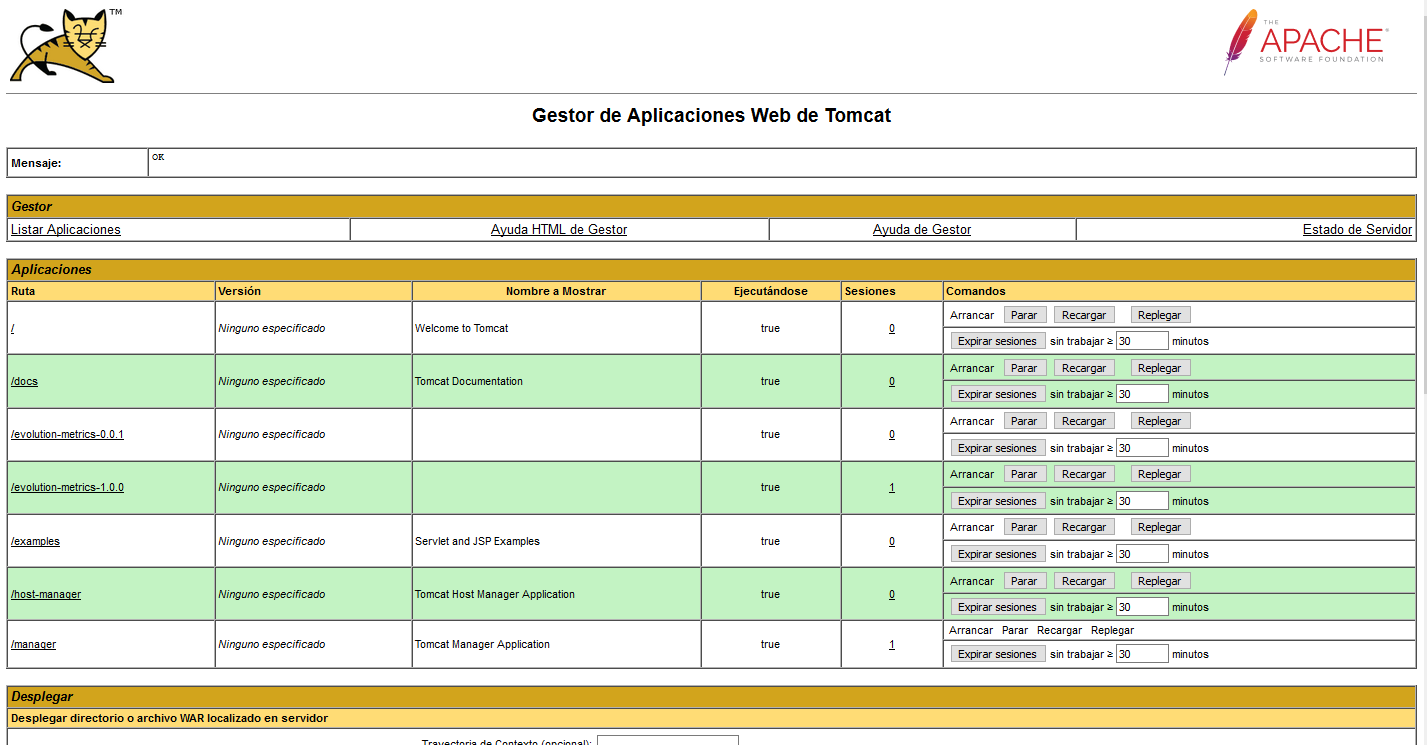
\includegraphics[scale=0.4]{M4_TomcatAppManager}
			\caption{Gestor de aplicaciones Tomcat con dos versiones desplegadas de la aplicación de este proyecto}\label{fig:M4_TomcatAppManager}
		\end{figure}
		\FloatBarrier
		
\end{description}
\subsection{Logging}
El proceso de logging permite registrar lo que ocurre dentro de la aplicación para poder identificar futuros problemas en tiempo de ejecución. Esto es especialmente útil en la fase de producción, después de haber desplegado la aplicación.
\begin{description}
	\item[SLF4J.] Fachada de logging.
	
		Enlace a página de descarga:
	
		\url{https://www.slf4j.org/download.html}
	
	\item[Log4j 2.] Logger. Se ha utilizado la versión  v2.11.2.
	
	 	Enlace a página de descarga:
	
	 	\url{https://logging.apache.org/log4j/2.x/download.html}
	
		SLF4J (\textit{Simple Logging Facade for Java}) es una capa intermedia entre el framework de logging como \textit{java.util.logging}, \textit{logback}, \textit{log4j}) y la aplicación, esto permite poder cambiar de framework de logging facilmente en tiempo de despliegue.
		
		Se utilizó Log4j al tener experiencia previa con esta herramienta. Esta herramienta permite configurar este proceso por medio de un fichero log4j2 con extensión XML, JSON, YAML o Properties\footnote{Manual de configuración de Log4j 2: \url{https://logging.apache.org/log4j/2.x/manual/configuration.html}} \cite{noauthor_log4j_nodate}. En este proyecto se configuró mediante un fichero con extensión \textit{.properties}. Para más información consultar el . 
		
		Ambas herramientas están integradas con Maven, añadiendo en el pom las dependencias correspondientes.
	
\end{description}
\subsection{Pruebas}
La fase de pruebas permite probar que la implementación que se ha estado llevando a cabo funciona correctamente. Se han realizado dos tipos de pruebas: unitarias y de integración. Las unitarias prueban los diferentes módulos y las de integración prueban la relación que tienen los diferentes módulos entre sí.
\begin{description}
	\item[JUnit5]. Conjunto de bibliotecas para el desarrollo de pruebas unitarias. 
	
		Se ha utilizado la versión  v5.3.1. Enlace a página de descarga:
		
		\url{https://junit.org/junit5/}
		
		JUnit es una herramienta que se utiliza para realizar pruebas unitarias de forma automática o semiautomática de aplicaciones Java. Se han ejecutado de ambas formas. La automatización completa ha sido posible gracias a las herramientas de CI (\textit{Continuous Integration}) de GitLab.
		Esta versión de JUnit 5, sobre la anterior JUnit 4, ha influido en este proyecto de la siguiente manera:
		\begin{itemize}
			\item JUnit 5 soporta \textbf{Java 11}.
			
			\item Permite realizar asertos (\textit{asserts}) de tipo \textit{\textbf{assertAll()}} \footnote{\url{https://junit.org/junit5/docs/current/api/org/junit/jupiter/api/Assertions.html}}. Se realizó en pruebas en versiones previas pero luego se optó por quitarlos y utilizar asertos simples.
			
			\item Permite realizar \textbf{comprobaciones de lanzamiento de excepciones} en asertos del tipo \textit{assertThrows()}.
			
			\item Permite realizar presunciones (\textit{\textbf{assumptions}}) que permiten realizar una comprobación que pasará por alto el test (lo marca como \textit{skipped}) si la comprobación falla. Es decir que no lo marcará como error, simplemente no realizará el test. \\Esto ha sido útil de cara a probar funciones que realicen conexiones a GitLab que requieran credenciales de acceso. No es correcto publicar en los test las credenciales de acceso del programador a GitLab. Por tanto estos test tienen presunciones que comprueban que se tiene las credenciales de acceso y no se realizan los test si no se dispone de estas credenciales, en lugar de lanzar un error por no poder realizar la conexión. Por tanto estos test se ejecutan manualmente por el programador en su equipo local y no se ejecutan automáticamente en el proceso de integración continua de GitLab.
			
			\item Permite crear \textbf{test parametrizados}. Estos son test que prueban funciones que requieren argumentos. Cada combinación de argumentos es un caso de prueba y crear un test para cada combinación es un caso claro del defecto de código: `código duplicado'. Por ello estos argumentos se pueden generar mediante funciones, enumeraciones, proveedores de argumentos o recolectar desde un CSV y solo ser necesario un test para todas las combinaciones de argumentos posibles.
		\end{itemize}
\end{description}
\subsection{Frameworks y librerías específicas para el proyecto}
%\todo Además de los enlaces de la aplicación añade los enlaces de tu repositorio
\begin{description}
	\item[gitlab4j-api]. Framework de conexión a GitLab API. 
	
		Se ha utilizado la versión  v4.9.14. Enlace:
		
		\url{https://github.com/gitlab4j/gitlab4j-api}
		
		Se ha preferido frente a \textit{timols/java-gitlab-api} \footnote{\url{https://github.com/timols/java-gitlab-api}} tras realizar un estudio sobre sus métricas de evolución y una comparativa sobre la documentación. Concluyendo en que \textbf{gitlab4j-api} contiene mejor documentación, mejor evolución y, a día de hoy, sigue evolucionando.
		
	\item[Apache Commons Math]. Librería que se utiliza para matemáticas descriptivas utilizada para el cálculo de cuartiles para obtener los valores umbrales de las métricas según las estadísticas. 
	
		Se ha utilizado la versión  v3.6.1. Enlace a página de descarga:
	
		\url{https://commons.apache.org/proper/commons-math/download_math.cgi}
		
		Ejemplo de uso:
		
\begin{lstlisting}
...
descriptiveStatisticsForMetric = new DescriptiveStatistics(
	datasetForMetric
	.stream()
	.mapToDouble(x -> x)
	.toArray());
q1ForMetric = descriptiveStatisticsForMetric
	.getPercentile(25);
q3ForMetric = descriptiveStatisticsForMetric
	.getPercentile(75);
...
\end{lstlisting}
\end{description}
\subsection{Interfaz gráfica}
\begin{description}
	\item[Vaadin]. Framework para desarrollo de interfaces Web con Java.
		Se ha utilizado la versión  v13.0.0 Enlace:
		
		\url{https://vaadin.com/}
		
		Con este framework no ha sido necesario escribir HTML, solo Java y un poco de CSS. Por ejemplo, para implementar un checkbox se utilizaría el siguiente código:
\begin{lstlisting}
...
Checkbox checkbox = new Checkbox();
checkbox.setLabel("Default Checkbox");
...
\end{lstlisting}
		y el resultado sería el se la Fig. \ref{fig:M4_Vaadin_ChkBox}
\begin{figure}[!h]
	\centering
	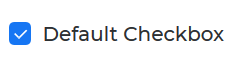
\includegraphics[scale=0.5]{M4_Vaadin_ChkBox}
	\caption{Checkbox generado por Vaadin}\label{fig:M4_Vaadin_ChkBox}
\end{figure}
\FloatBarrier

\end{description}
\subsection{CI/CD y revisión automática}
\begin{description}
	\item[GitLab]. Plataforma de desarrollo colaborativo y forja de repositorios en la que se ha almacenado el proyecto en un repositorio Git.
	
		Enlace a GitLab:
		
		\url{https://gitlab.com/users/sign_in}
		
		Enlace al repositorio del proyecto:
		
		\href{https://gitlab.com/mlb0029/comparador-de-metricas-de-evolucion-en-repositorios-software}{https://gitlab.com/mlb0029/comparador-de-metricas-de-evolucion-en-repositorios-software}
		
		Para más información hay una comparativa entre GitHub y GitLab en la sección \ref{sect:3_2_1_GitHubVSGitLab}.
		
	\item[Codacy]. Herramienta de generación automática de informes de calidad de código.
	
		 Enlace a Codacy:
		 
		 \url{https://www.codacy.com/}
		 
		 Enlace a proyecto en Codacy: 
		 
		 \href{https://app.codacy.com/project/mlb0029/comparador-de-metricas-de-evolucion-en-repositorios-software/dashboard}{https://app.codacy.com/project/mlb0029/comparador-de-metricas-de-evolucion-en-repositorios-software/dashboard}
	
	\item[JaCoCo]. Librería para cobertura de código en Java utilizada para enviar información de cobertura a Codacy.
	
		Se ha utilizado la versión v0.8.3.
		
		Enlace:
		
		\url{https://www.eclemma.org/jacoco/}
	
	\item[Heroku]. Herramienta para despliegue continuo (CD).
	
		Enlace a herramienta:
		
		\url{https://id.heroku.com/login}
		
		Enlace a aplicación desplegada:
		
		\url{https://evolution-metrics.herokuapp.com/}
	
\end{description}
\subsection{Documentación}
\begin{description}
	\item[LaTeX]. Sistema de composición de textos.
		Enlace a herramienta:
		
		\url{https://www.latex-project.org/}
		
	\item[TeXstudio]. Entorno de desarrollo de documentos LaTeX.
	
		Enlace a herramienta:
		
		\url{https://www.texstudio.org/}
	
	\item[Zotero]. Herramienta de gestión de fuentes bibliográficas.
		
		Enlace a herramienta:
		
		\url{https://www.zotero.org/}
	
\end{description}
\subsection{Técnicas}
\begin{itemize}
	\item A lo largo del proyecto se han utilizado numerosos patrones de diseño \cite{gamma_patrones_2002} como Singleton, Factory Method, Wrapper, Builder, Listener, etc. Se detallará más sobre esto en los apéndices.
	
	\item Para el motor de métricas se ha utilizado como base el framework propuesto en \textit{Soporte de Métricas con Independencia del Lenguaje para la Inferencia de Refactorizaciones} \cite{marticorena_soporte_2005}. Ver Fig. \ref{fig:MCTMotorMetricas} en la sección \ref{sect:3_3_3_FrameworkMedicion}.
	
	\item El ciclo de vida del software de este proyecto ha seguido un modelo de proceso iterativo e incremental: Scrum \cite{noauthor_scrum_2019}. Este proceso de detalla en `Apéndice A - Plan de Proyecto Software'. \todo Referencia a apéndice?
\end{itemize}

%herramientas codacy maven, gitlab, capturas, etc, cobertura, heroku, ci, pipeline, token...